\documentclass[12pt]{report}

\newcommand\htmladdnormallink[2]{\href{#2}{#1}}

\textheight 22cm
\textwidth 15.5cm
\oddsidemargin 0pt\evensidemargin 0pt
%\oddsidemargin 14pt\evensidemargin 0pt
%\topmargin -40pt
\topmargin-30pt
%\bottommargin0pt
\def\baselinestretch{1.1}
%\addtolength{\parskip}{1ex}
\jot=.5ex
%\parskip = 0.02in


\setlength\arraycolsep{2pt}



\usepackage{amssymb}
\usepackage{amsmath,bm}
\usepackage{amssymb}
\usepackage{graphicx}
\graphicspath{ {../fig/}}
\usepackage{amsfonts}         
\usepackage{fancybox}   

%\usepackage[numbers]{natbib}

\usepackage{enumitem}

\usepackage{slashed}




\usepackage[usenames,dvipsnames]{xcolor}%http://en.wikibooks.org/wiki/LaTeX/Colors

\definecolor{darkgreen}{rgb}{0,0.4,0}
\definecolor{darkred}{rgb}{0.4,0,0}
\definecolor{darkblue}{rgb}{0,0,0.4}
\definecolor{lightblue}{rgb}{.6,.6,0.9}
\newcommand{\cobl}{\color{darkblue}}

\newcommand{\cor}{\color{red}}
\newcommand{\cog}{\color{darkgreen}}
\newcommand{\cob}{\color{black}}

\definecolor{uglybrown}{rgb}{0.8,  0.7,  0.5}

\def\ii{{\bf i}}
\def\Ione{\mathbb{I}}
\def\UU{{\bf U}}
\def\HH{{\bf H}}
\def\pp{{\bf p}}
\def\aa{{\bf a}}
\def\qq{{\bf q}}
\def\eps{\epsilon}
\def\half{{1\over 2}}
\def\Tr{{{\rm Tr~ }}}
\def\tr{{\rm tr}}
\def\Re{{\rm Re\hskip0.1em}}
\def\Im{{\rm Im\hskip0.1em}}
\def\ppi{\boldsymbol{\pi}}
\def\pphi{\boldsymbol{\phi}}
%\def\pphi{\phi}
\def\grad{\vec \nabla}
\def\vB{\vec B}
\def\vE{\vec E}
\def\vA{\vec A}
\def\vAA{ \vec{\bf A}}
\def\vEE{{{\vec {\bf E}}}}
\def\vBB{{\vec {\bf B}}}

\def\CL{{\cal L}}



\def\bra#1{\left\langle#1\right|}
\def\ket#1{\left|#1\right\rangle}
\def\bbra#1{{\langle\langle}#1|}
\def\kket#1{|#1\rangle\rangle}
\def\vev#1{\left\langle{#1}\right\rangle}

\def\ketbra#1#2{ | #1 \rangle\hskip-2pt\langle #2|}



\def\be{\begin{equation}}
\def\ee{\end{equation}}
\def\({\left(}
\def\){\right)}



\newcommand{\bea}{\begin{eqnarray}}
\newcommand{\eea}{\end{eqnarray}}


\def\parfig#1#2{
\parbox{#1\textwidth}
{\includegraphics[width=#1\textwidth]{#2}}
}



%%from  Rudro Rana Biswas
\usepackage[pagebackref,  % this puts links to the page numbers where refs appear
%pdftex, 
bookmarks={false}, pdfauthor={John McGreevy}, pdftitle={Yay, physics!}]{hyperref}
\hypersetup{colorlinks=true, 
linkcolor=BrickRed, 
citecolor=Violet, 
filecolor=OliveGreen, 
urlcolor=RoyalBlue, 
filebordercolor={.8 .8 1}, 
urlbordercolor={.8 .8 0}}%http://en.wikibooks.org/wiki/LaTeX/Hyperlinks


%\usepackage{mathtools} % for inclusion arrow \xhookrightarrow{}


\renewcommand{\theequation}{\arabic{equation}}
\newif{\ifeq}           % defines a new condition @eq tested by the conditional \ifeq
\eqtrue                 % if uncommented, declares @eq to be true
%\eqfalse              % if uncommented, declares @eq to be false
%                                %
%                                % to use this, wrap text with the conditional, eg:
%                                %
%                                % \ifeq
%                                % SHOW THIS IFF \eqtrue HAS BEEN DECLARED
%                                % \fi
%
\def\answer#1
{
\ifeq
\textcolor{darkblue}{#1}
\fi
}

\begin{document}
\begin{center}

University of California at San Diego -- 
Department of Physics --
Andy Wan

{\Large\bf  Physics 210B Non-equilibrium  Fall 2025}\\
{\Large\bf Assignment 1 \answer{--~~~ Solutions} }
\end{center}


\noindent
\hfill {\bf Due 11:59pm {Monday, October 6, 2025}} 


%I will add another problem later today.
\bigskip
\hrule




\begin{enumerate}

\item Is there a topic for which you would be disappointed if you didn't learn about it in 210B?  

\answer{I would love to see some fluid dynamics. I also really like the idea to work on those simulations.}

\item {\bf Brain-warmer: A random walk in $d>1$ dimensions.}
\begin{enumerate}
\item Consider a random walk in two dimensions where at each time increment the walker takes a step by $\vec x_i = \ell ( \cos \theta_i, \sin\theta_i)$
for some fixed length $\ell$, where $\theta_i$ is chosen from the uniform distribution on $[0, 2\pi)$.  
Define the mean-square displacement $ \vev{ \vec X^2 }$, where $\vec X \equiv \sum_{i=1}^t \vec x_i$.
Show that $\vev{\vec X^2}$ grows linearly with $t$.  

\answer{
	\begin{equation}
		\vec X = \ell \sum_{i=1}^t (\cos \theta_i, \sin \theta_i)
	\end{equation}
	\begin{equation}
		\vev{ \vec X^2 } = \ell^2 \left( \sum_{i=1}^t \sum_{j=1}^t (\cos \theta_i, \sin \theta_i) \cdot (\cos \theta_j, \sin \theta_j) \right)
	\end{equation}
	\begin{equation}
		= \ell^2 t + \ell^2 \sum_{i \neq j} (\cos \theta_i, \sin \theta_i) \cdot (\cos \theta_j, \sin \theta_j)
		= \ell^2 t + 2\ell^2 \sum_{1 \leq i < j \leq t} (\cos \theta_i, \sin \theta_i) \cdot (\cos \theta_j, \sin \theta_j) 
	\end{equation}
	\begin{equation}
		= \ell^2 t + 2\ell^2 \sum_{1 \leq i < j \leq t} \cos(\theta_i - \theta_j)
		= \ell^2 t 
	\end{equation}
Clearly, the cross terms vanish because $\theta_i$ and $\theta_j$ are independent and uniformly distributed on $[0, 2\pi)$, so $\vev{\cos(\theta_i - \theta_j)} = 0$. $\vev{ \vec X^2 }$ grows linerly with $t$. 
}

\item Convince me that the same idea works in any number of dimensions, where now the directions are chosen uniformly on the unit sphere in $d-1$ dimensions,
that is, the increment is $ \vec x_i = \ell \hat n_i$.

\answer{
	\begin{equation}
		\vec X = \ell \sum_{i=1}^t \hat n_i
	\end{equation}
	\begin{equation}
		\vev{ \vec X^2 } = \ell^2 \left( \sum_{i=1}^t \sum_{j=1}^t \hat n_i \cdot \hat n_j \right)
	\end{equation}
	\begin{equation}
		= \ell^2 t + \ell^2 \sum_{i \neq j} \hat n_i \cdot \hat n_j
		= \ell^2 t + 2\ell^2 \sum_{1 \leq i < j \leq t} \hat n_i \cdot \hat n_j 
	\end{equation}
	\begin{equation}
		= \ell^2 t + 2\ell^2 \sum_{1 \leq i < j \leq t} \cos(\theta_{ij})
		= \ell^	2 t 
	\end{equation}	
where $\theta_{ij}$ is the angle between $\hat n_i$ and $\hat n_j$. The cross terms vanish because $\hat n_i$ and $\hat n_j$ are independent and uniformly distributed on the unit sphere in $d-1$ dimensions, so $\vev{\cos(\theta_{ij})} = 0$. $\vev{ \vec X^2 }$ grows linerly with $t$.	
}


\item 
Now suppose that the lengths $\ell$ of the steps are sampled from a distribution $g(\ell)$, say $g(\ell) = {1\over \lambda} e^{ - \ell/\lambda}$.  
Show that the result still holds.
\answer{
	\begin{equation}
		\vev{ \vec X^2 } = \left( \sum_{i=1}^t \sum_{j=1}^t l_i \hat n_i \cdot l_j \hat n_j \right)
	\end{equation}
	\begin{equation}
		= \sum_{i=1}^t l_i^2 + \sum_{i \neq j} l_i l_j \hat n_i \cdot \hat n_j
		= \sum_{i=1}^t l_i^2 + 2\sum_{1 \leq i < j \leq t} l_i l_j \hat n_i \cdot \hat n_j 
	\end{equation}
	\begin{equation}
		= \sum_{i=1}^t l_i^2 + 2\sum_{1 \leq i < j \leq t} l_i l_j \cos(\theta_{ij})
		= \sum_{i=1}^t l_i^2  
	\end{equation}
	\begin{equation}
		\vev{ \vec X^2 } = t \vev{l^2} = 2t \lambda^2
	\end{equation}
}



\end{enumerate}





\end{enumerate}

Comment on simulations: 
One of the great joys of being away from equilibrium is that things depend on time and we can watch them move around by simulating their dynamics.
So we are going to do some simulations in this class.
You can use whatever software you like.  I prefer to use Julia (download \href{https://julialang.org/install/}{here})
via the very convenient interface VS Code (download \href{https://code.visualstudio.com/}{here}).  
Please email me if you have any trouble that isn't easily answered by asking the internets.

\begin{enumerate}[resume]




\item {\bf Some simulations of random walks.}

\begin{enumerate}
\item 
Simulate an ordinary 1d random walk with fixed step size.
Get enough statistics to see that 
the mean-square displacements grow with time $\vev{\Delta X^2 } \propto  t$.  

Check the prediction of the Central Limit Theorem, i.e.~that the distribution for the mean displacement is Gaussian.
Here is one way to check %numerically that your distribution for the mean is Gaussian:
this numerically:
divide up a long walk into a collection of blocks whose size is larger than the correlation time.  
Then plot a histogram of the block lengths and fit it to a Gaussian.

\answer{
	\begin{figure}[h]
		\centering
		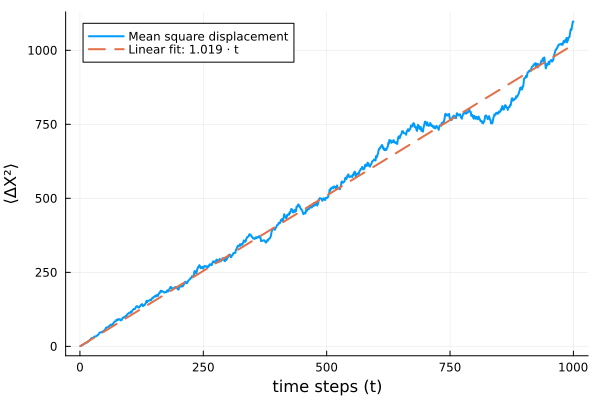
\includegraphics[width=0.6\textwidth]{walk1D_100trials.png}
		\caption{1D random walk with 1000 steps and 100 trials.}
	\end{figure}
	\begin{figure}[h]
		\centering
		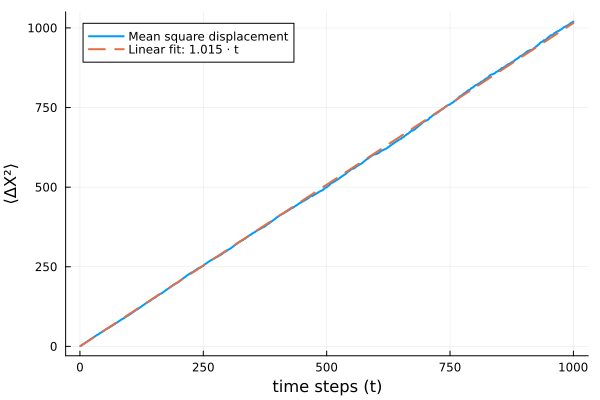
\includegraphics[width=0.6\textwidth]{walk1D_10000trials.png}
		\caption{1D random walk with 1000 steps and 10000 trials.}
	\end{figure}
}

\item Introduce weak correlations between the steps and check that the CLT still holds.  

\answer{
	\begin{figure}[h]
		\centering
		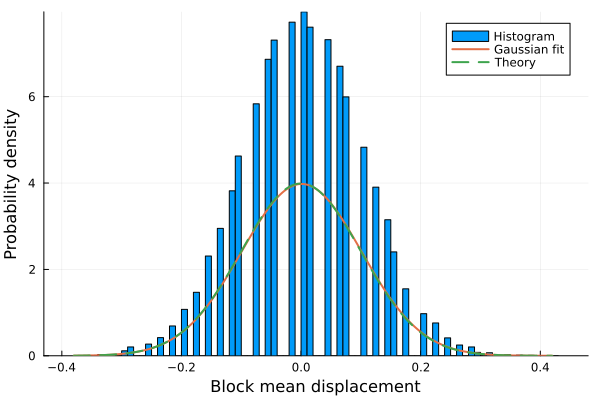
\includegraphics[width=0.6\textwidth]{clt.png}
		\caption{CLT with uncorrelated increments.}
	\end{figure}
}
Here are two ways to introduce short-time correlations in the steps $s_n$ of our random walk $X(t) = \sum_{n=1}^t s_n $: \\
(1) Choose a set of iid increments $\eta_i, i=1:N$ all at once. Then define the step to be 
\be s_n = \sum_{j=1}^q a_j \eta_{n-j} \ee
where $a_j$ is a set of $q$ numbers you pick
(and $\eta_{i} = 0 $ for $i<1$ or $i>N$).  
This is called `finite-memory moving average', and will induce correlations over a time $q$.

(2) Sample the increments $s_n$ from an ``Ornstein-Uhlenbeck process", that is: 
\be s_{n+1} = \rho s_n + \eta_n \ee
where $\rho$ (with $|\rho| < 1$) is a parameter and $\eta_n$ is some iid Gaussian noise with variance $\sigma_\eta = \sqrt{ 1 - \rho^2}$.
Here are the key steps in Julia: 
\begin{verbatim}
s = zeros(N)
s[1] = randn()
for n in 2:N 
	s[n] = rho * s[n-1] + randn() * sigma_eta
end
\end{verbatim}

Is the distribution still Gaussian?  Convince me.
\answer{
	\begin{figure}[h]
		\centering
		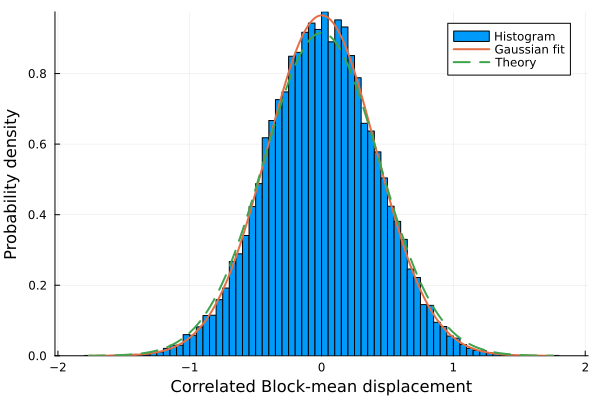
\includegraphics[width=0.6\textwidth]{clt_correlated_distribution.png}
		\caption{CLT with correlated increments.}
	\end{figure}\\
Yes, the distribution is still Gaussian. See figure 4.
}

%\item Simulate a 1d continuous-time random walk (CTRW).  
%
%{\cor this is best done using the Gillespie algorithm.}

\item{} [Bonus problem] Simulate a self-avoiding walk.  
Keep track of the whole history of the walk.  Define some small distance of minimal approach.
At each candidate step, make sure that it is not getting too close to a previous location before you accept.  \hfill [continued on next page]

Can you see a difference in the RMS displacement versus number of steps?  

[Note that this may not be (is not) the best way to simulate such a correlated walk.  If you think of a better way, such as keeping track of a grid of visited sites, please feel free to do that instead.]



\end{enumerate}


\end{enumerate}
\end{document}